% !TeX encoding = UTF-8

\documentclass{protokol}

\usepackage{pdfpages}
\usepackage{tikz}
\usetikzlibrary{calc}
\usetikzlibrary{arrows}

%====== Units =====
\usepackage{siunitx}
\sisetup{inter-unit-product =\ensuremath{\cdot}}
\sisetup{group-digits = integer}
\sisetup{output-decimal-marker = {,}}
\sisetup{exponent-product = \ensuremath{\cdot}}
\sisetup{separate-uncertainty}
\sisetup{tight-spacing = false}
%\sisetup{scientific-notation = true}
%\sisetup{round-mode=places,round-precision=4}
%\sisetup{evaluate-expression}


%====== Grafy =====
\usepackage{pgfplots}
\pgfplotsset{width=0.8\linewidth, compat=1.17}
\def\plotcscale{0.8}
\usepackage{pgfplotstable}
\usepackage[figurename=Obr.]{caption} % figure caption rename

%====== Rovnice align block ======
\usepackage{amsmath}
\setlength{\jot}{10pt} % rozestup mezi řádky

\graphicspath{ {./img/} }

%====== Vyplňte údaje ======
\jmeno{Jakub Charvot}
\kod{240844}
\rocnik{3.}
\obor{MET}
\skupina{MET/2}
\spolupracoval{--}

\merenodne{4.3.\ 2024}
\odevzdanodne{17.3.\ 2024}
\nazev{Proudová zrcadla}
\cislo{2} %měřené úlohy

\predmet{Návrh analogových integrovaných obvodů}
\ustav{Ústav mikroelektroniky}
\skola{FEKT VUT v~Brně}

\def\para{x+0}
\def\parb{\para-80}


%citace 
\usepackage[backend=biber, style=iso-numeric, sortlocale=cs_CZ, autolang=other, language=czech]{biblatex}
\addbibresource{bibliography.bib}
\DeclareFieldFormat{labelnumberwidth}{\mkbibbrackets{#1}}
% hyperlinky
\usepackage[colorlinks]{hyperref}

% odstavce
\usepackage{parskip}

% Bloky kódu
\usepackage{xcolor}

%New colors defined below
\definecolor{codegreen}{rgb}{0,0.6,0}
\definecolor{codegray}{rgb}{0.5,0.5,0.5}
\definecolor{codepurple}{rgb}{0.58,0,0.82}
\definecolor{backcolour}{rgb}{0.95,0.95,0.92}

\usepackage{listings}
\lstdefinestyle{mystyle}{
  backgroundcolor=\color{backcolour}, commentstyle=\color{codegreen},
  keywordstyle=\color{magenta},
  numberstyle=\tiny\color{codegray},
  stringstyle=\color{codepurple},
  basicstyle=\ttfamily\footnotesize,
  breakatwhitespace=false,         
  breaklines=true,                 
  captionpos=b,                    
  keepspaces=true,                 
  numbers=left,                    
  numbersep=5pt,                  
  showspaces=false,                
  showstringspaces=false,
  showtabs=false,                  
  tabsize=2
}
\lstset{
	inputencoding=utf8,
	extendedchars=true,
	literate={á}{{\'a}}1 {č}{{\v{c}}}1 {ď}{{\v{d}}}1 {é}{{\'e}}1 {ě}{{\v{e}}}1 
           {í}{{\'i}}1 {ň}{{\v{n}}}1 {ó}{{\'o}}1 {ř}{{\v{r}}}1 {š}{{\v{s}}}1 
           {ť}{{\v{t}}}1 {ú}{{\'u}}1 {ů}{{\r{u}}}1 {ý}{{\'y}}1 {ž}{{\v{z}}}1 
           {Á}{{\'A}}1 {Č}{{\v{C}}}1 {Ď}{{\v{D}}}1 {É}{{\'E}}1 {Ě}{{\v{E}}}1 
           {Í}{{\'I}}1 {Ň}{{\v{N}}}1 {Ó}{{\'O}}1 {Ř}{{\v{R}}}1 {Š}{{\v{S}}}1 
           {Ť}{{\v{T}}}1 {Ú}{{\'U}}1 {Ů}{{\r{U}}}1 {Ý}{{\'Y}}1 {Ž}{{\v{Z}}}1,
	style=mystyle
	}

% Číslování
\pagenumbering{arabic}

% =========================================
% =============== DOKUMENT ================
% =========================================
\begin{document}
	%====== Vygenerování tabulky ======
	\maketitle

\section{Vypracování}

\begin{figure}[h!]
  \centering
  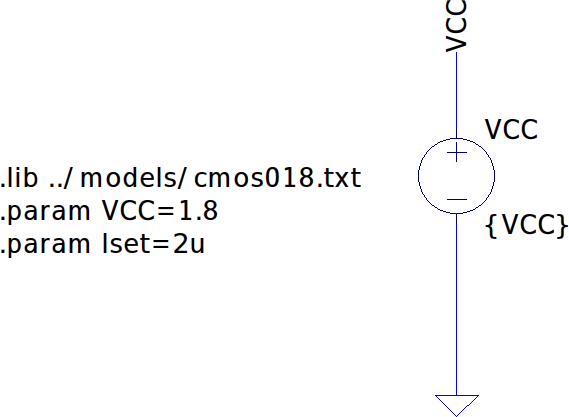
\includegraphics[scale=0.4]{spice0.png}
  \caption{Společná část SPICE kódu a napájecí zdroj.}
  \label{fig:spice0-png}
\end{figure}

\subsection{Jednoduché proudové zrcadlo}
\begin{figure}[h!]
  \centering
  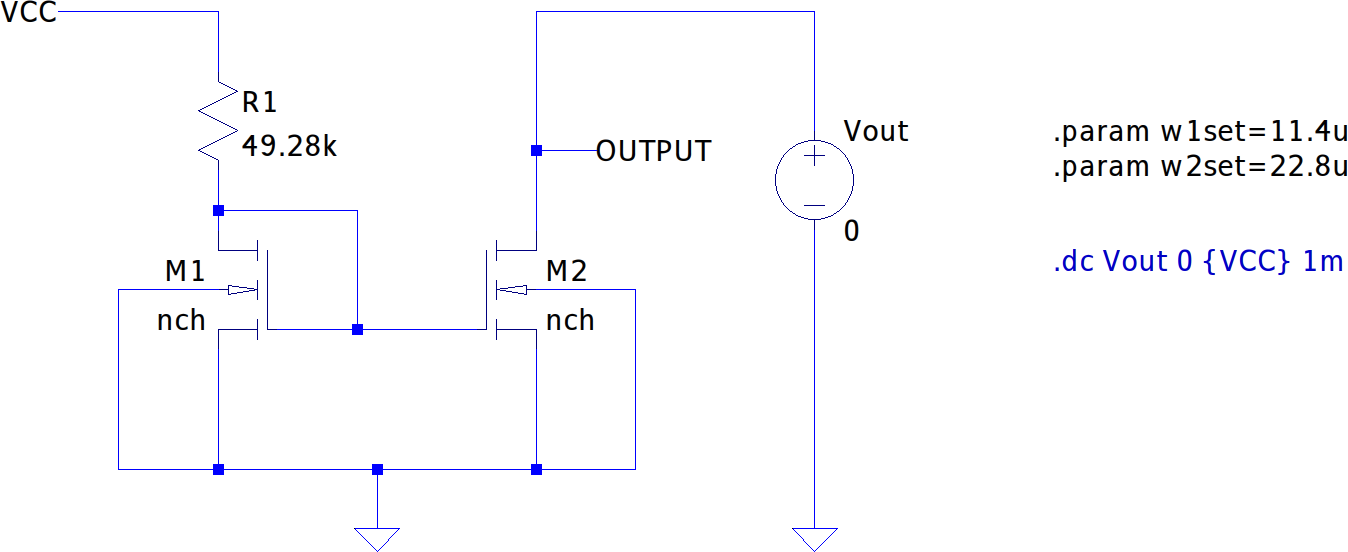
\includegraphics[scale=0.4]{spice1.png}
  \caption{Zapojení a SPICE kód.}
  \label{fig:spice1-png}
\end{figure}
\subsubsection{Ruční návrh}
\[
    I_D=\frac{1}{2} \cdot K P_N \cdot \frac{W}{L} \cdot\left(U_{G S}-U_{T H}\right)^2
\]
\[
    \frac{W}{L}=\frac{2\cdot I_{D}}{KP_{N}\cdot (U_{GS} -U_{TH})^2 } 
\]
\[
    \frac{W_{1} }{L_{1} }=\frac{2\cdot \num{25e-6}}{\num{220e-6}\cdot (\num{0.2})^2 } 
\]
\[
    \frac{W_{1} }{L_{1} }\doteq \num[round-mode=places,round-precision=2]{5.681818181818182} 
\]
Pro oba tranzistory zvolíme stejnou délku kanálu \(L_{1}=L_{2} = \qty{2}{\micro\meter}\), tedy \(W_{1} =\qty[round-mode=places,round-precision=2]{11,36363636363636}{\micro\meter}\). Druhý tranzistor má dosáhnout dvakrát vyššího proudu, takže zvolíme \(W_{2} =\qty{22,72}{\micro\meter}\).

\[
    R_1=\frac{U_R}{I_{M 1}}=\frac{U_{C C}-U_{G S 1}}{I_{M 1}}=\frac{U_{C C}-\left(U_{T H 0,1}+U_{O V, 1}\right)}{I_{M 1}}
\]
\[
    R_1=\frac{\num{1.8}-\left(\num{368,024e-3}+\num{0.2}\right)}{\num{25e-6}}
\]
\[
    R_{1} \doteq \qty{49,28}{\kilo\ohm}
\]

Výstupní odpor tohoto zapojení je roven výstupnímu odporu tranzistoru \(M2\): 
\[
    r_{O U T}=\frac{1}{\lambda \cdot I_{M 2}}
\]

\[
    r_{O U T}=\frac{1}{\num[round-mode=places,round-precision=3]{0,0437895} \cdot \num{50e-6}}
\]
\[
    r_{O U T}=\qty[round-mode=places,round-precision=3]{454,5454545454545}{\kilo\ohm}
\]

\subsubsection{Výstupní charakteristika}
\begin{figure}[h!]
    \centering
    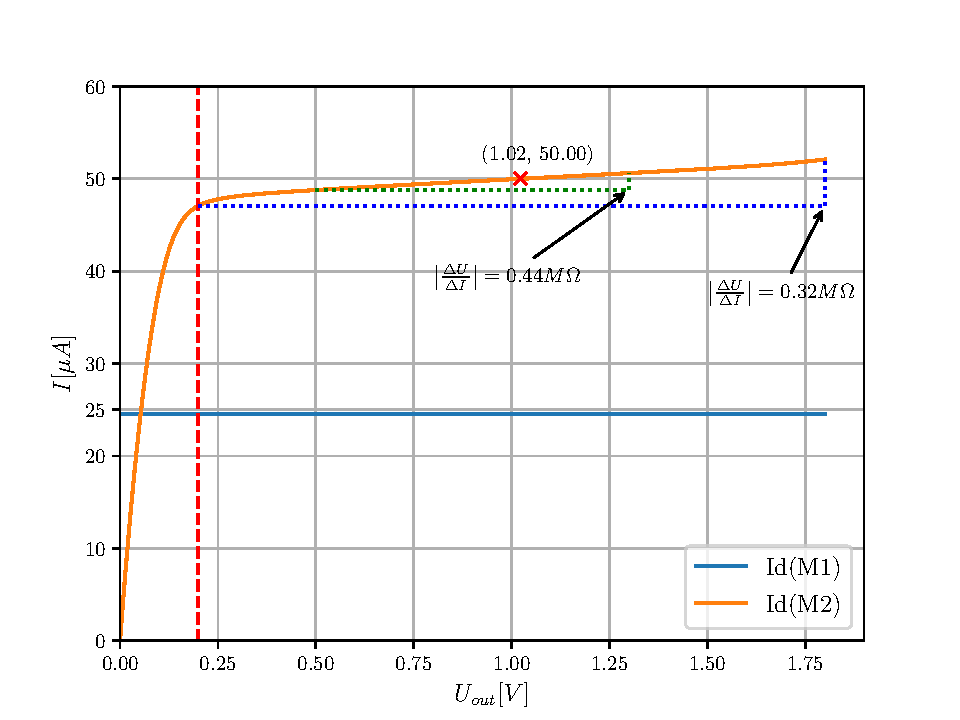
\includegraphics[width=0.8\textwidth]{2-1.pdf}
    \caption{DC analýza pro jednoduché proudové zrcadlo.}
    \label{fig:2-1-pdf}
\end{figure}



  \clearpage
  
\subsection{Kaskodové proudové zrcadlo}
\begin{figure}[h!]
  \centering
  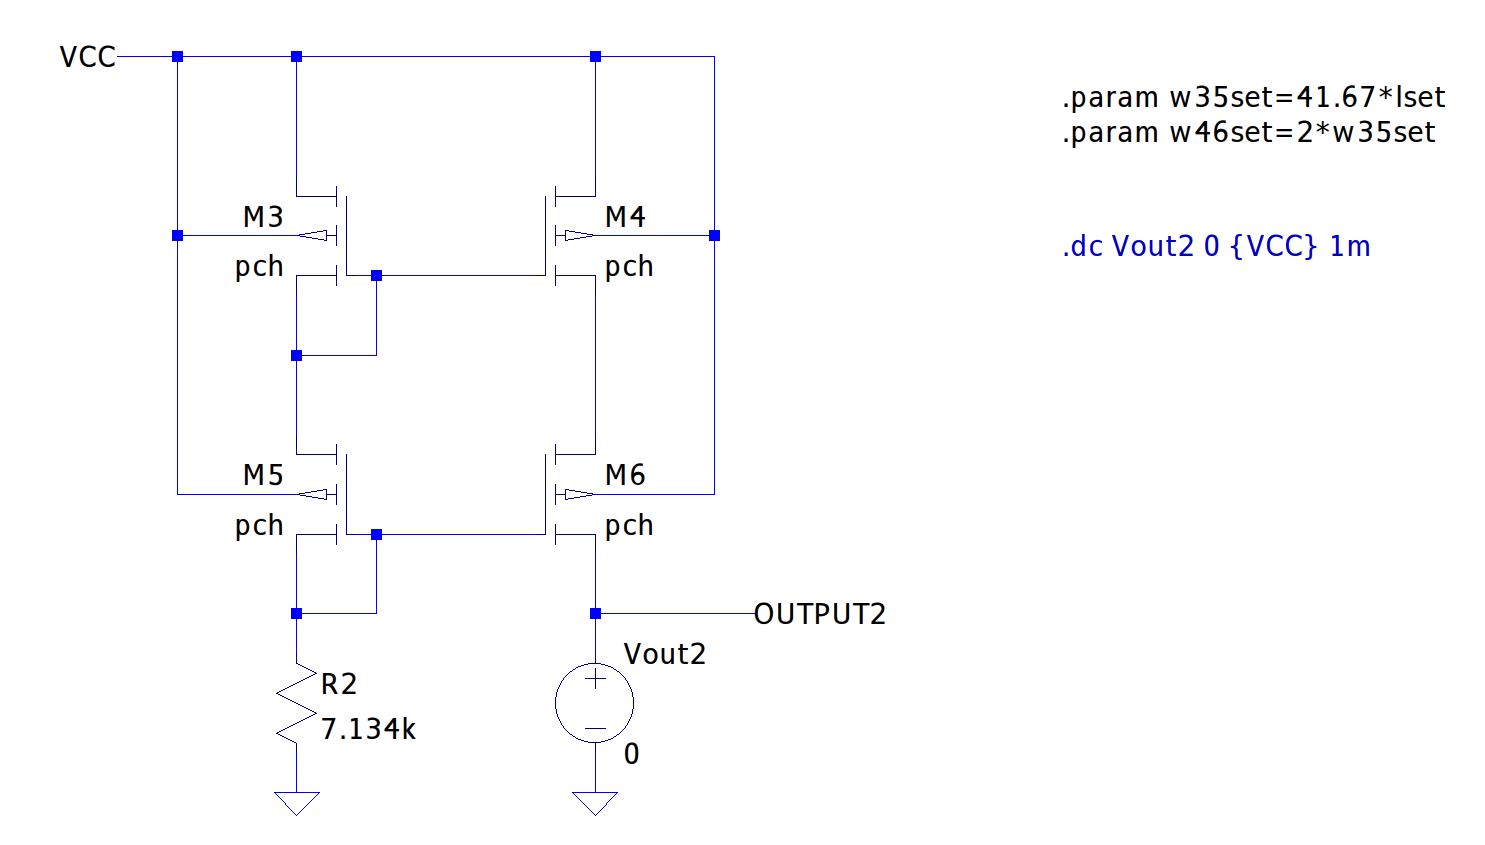
\includegraphics[scale=0.4]{spice2.png}
  \caption{Zapojení a SPICE kód.}
  \label{fig:spice2-png}
\end{figure}
\subsubsection{Ruční návrh}
Pro vstupní větev je stanoven proud \qty{50}{\micro\ampere}, výpočet rozměrů je proveden obdovným způsobem jako v minulém přkladu:
\[
    \frac{W_{3,5}}{L_{3,5}}=\frac{2\cdot I_{D3}}{KP_{P}\cdot (U_{GS} -U_{TH})^2 } 
\]
\[
    \frac{W_{3,5}}{L_{3,5}}=\frac{2\cdot \num{50e-6}}{\num{60e-6} \cdot (\num{0.2})^2 } 
\]
\[
    \frac{W_{3,5}}{L_{3,5}}=\num{41,67}
\]

Opět použijeme délku kanálu \(L_{3,5}=L_{4,6} = \qty{2}{\micro\meter}\), tedy \(W_{3,5} =\qty[round-mode=places,round-precision=2]{83,34}{\micro\meter}\). Druhý tranzistor má dosáhnout dvakrát vyššího proudu, takže zvolíme \(W_{4,6} =\qty{166,68}{\micro\meter}\)  

Pro nastavení proudu slouží rezistor R2. Jeho hodnota je stanovena na základě úbytku napětí na rezistoru.
% U_bs pro M3 je U_GS1 coz je U_th0 + U_ov
% z tabulky pak odecitam radek pro nejvyssi U_bs, coz je porad mene...
% zaokrouhleno nahoru 600m
\begin{align*}
    U_{R 2}=&U_{C C}-U_{G S 3}-U_{G S 5} \\
           =&U_{C C}-U_{T H 0,3}- U_{O V 3}-U_{T H, 5}-U_{O V 5} \\
           =&U_{C C}-U_{T H 0,3}-U_{T H, 5}-2 \cdot U_{O V 3,5} \\
           =&\num{1.8}-\num{0.4433}-\num{0.6}-2 \cdot \num{0.2} \\
           =&\qty{0.3567}{\volt}
\end{align*}

\begin{align*}
    R_{2} =& \frac{U_{R1}}{I_{M1} } \\
          =& \frac{\num{0.3567}}{\num{50e-6}} \\
          =& \qty{7.134}{\kilo\ohm}
\end{align*}

Pro výpočet výstupního odporu použijeme zjednodušený vztah, jelikož rozměry tranzistorů \(M4\) a \(M6\) jsou stejné:
\begin{align*}
    r_{OUT} =& r_{o4,6}^2 \cdot g_{m6} \\
            =& \left(\frac{1}{\lambda_{PMOS} \cdot I_{M6} }\right)^2 \cdot \frac{2\cdot I_{M6}}{U_{OV6} } \\
            =& \frac{2}{\lambda_{PMOS}^2 \cdot I_{M6} \cdot U_{OV6} } \\
            =& \frac{2}{\num{0.079}^2 \cdot \num{100e-6} \cdot \num{0.2}} \\
            =& \qty{16.02}{\mega\ohm}
\end{align*}

\subsubsection{Výstupní charakteristika}
\begin{figure}[h!]
    \centering
    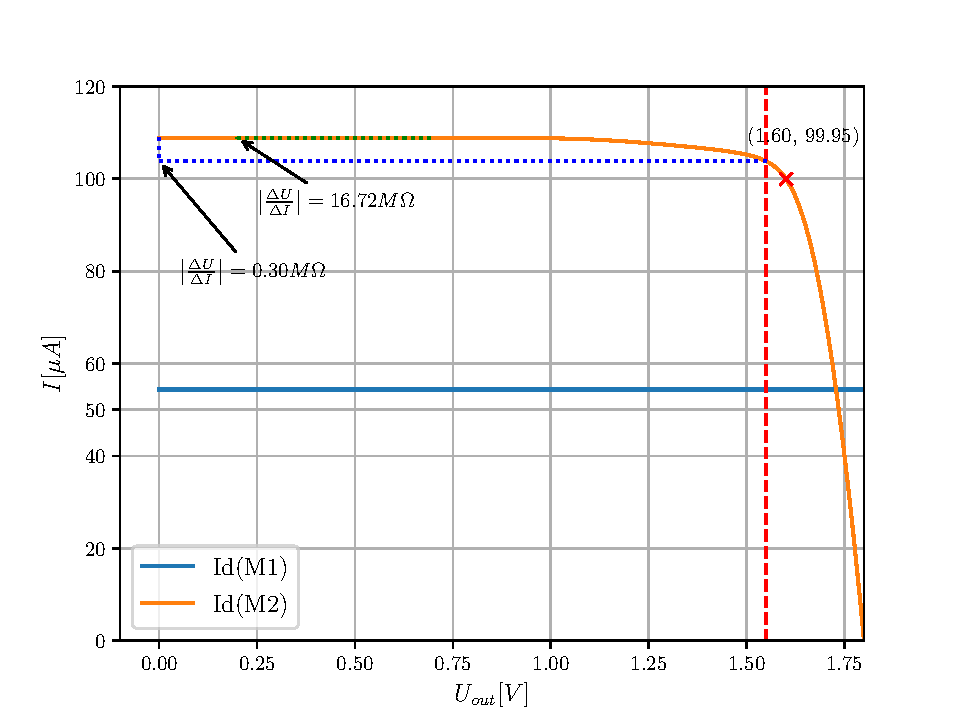
\includegraphics[width=0.8\textwidth]{2-2.pdf}
    \caption{DC analýza pro kaskodové proudové zrcadlo.}
    \label{fig:2-2-pdf}
\end{figure}

\clearpage
  
\subsection{Modifikované Wilsonovo proudové zrcadlo}
\begin{figure}[h!]
  \centering
  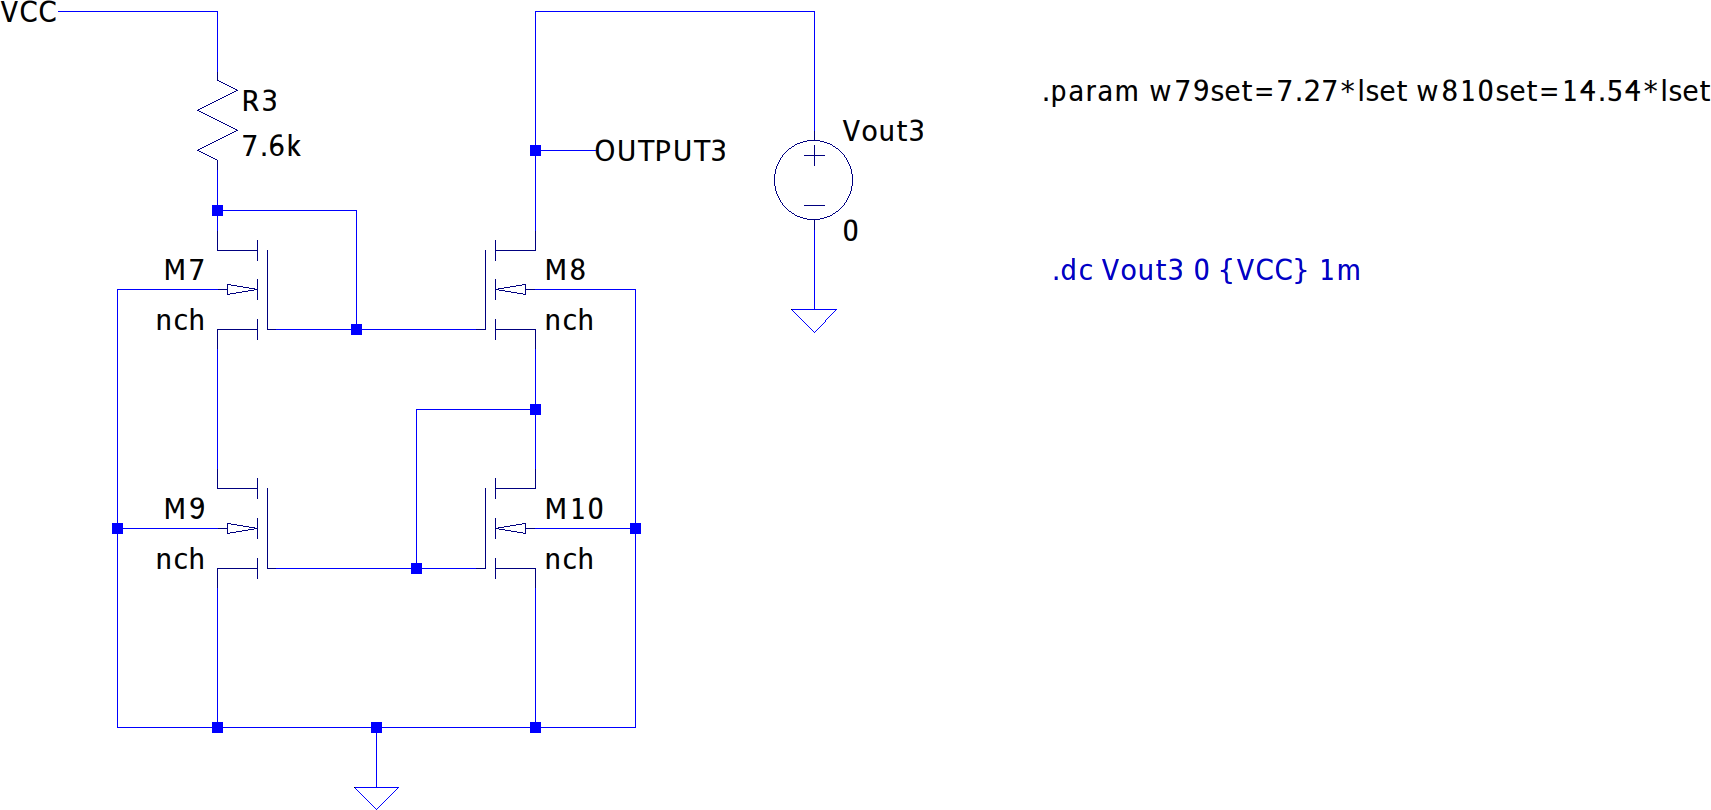
\includegraphics[scale=0.4]{spice3.png}
  \caption{Zapojení a SPICE kód.}
  \label{fig:spice3-png}
\end{figure}
\subsubsection{Ruční návrh}
Výpočet rozměrů tranzistorů vychází ze stejných rovnic jako v předešlých příkladech, délku kanálu zvolíme opět stejnou, tedy \(L_{7,9}=L_{8,10} = \qty{2}{\micro\meter}\). 

Pro vstupní větev je stanoven proud \qty{50}{\micro\ampere}, pro výstupní větev \qty{100}{\micro\ampere} a \(U_{OV} =\qty{0.25}{V}\):
\begin{align*}
    \frac{W_{7,9}}{L_{7,9}}=&\frac{2\cdot I_{D7}}{KP_{N}\cdot (U_{GS} -U_{TH})^2}\\
          =&\frac{2\cdot \num{50e-6}}{\num{220e-6} \cdot (\num{0.25})^2 } \\
          =&\num{7.27}
\end{align*}

Pak \(W_{7,9} =\qty{14.55e-06}{\micro\meter}\). Pro výstupní větev je proud dvojnásobný, tedy i šířka kanálu musí být \(W_{8,10}=2\cdot W_{7,9}=\qty{29,1}{\micro\meter}\).


Pro nastavení proudu slouží rezistor \(R3\). Jeho hodnota je stanovena na základě úbytku napětí na rezistoru.
% U_bs pro M7 je U_GS9 coz je U_th0 + U_ov
% z tabulky pak odecitam radek pro nejvyssi U_bs, coz je porad mene...
% zaokrouhleno nahoru 550m
\begin{align*}
    U_{R 3}=&U_{C C}-U_{G S 7}-U_{G S 9} \\
           =&U_{C C}-U_{T H 7}- U_{O V 7}-U_{TH0, 9}-U_{O V 9} \\
           =&U_{C C}-U_{T H 7}-U_{TH0, 9}-2 \cdot U_{O V 7,9} \\
           =&\num{1.8}-\num{0.55}-\num{0.37}-2 \cdot \num{0.25} \\
           =&\qty{0.38}{\volt}
\end{align*}

\begin{align*}
    R_{2} =& \frac{U_{R3}}{I_{M7} } \\
          =& \frac{\num{0.38}}{\num{50e-6}} \\
          =& \qty{7.6}{\kilo\ohm}
\end{align*}

Pro výpočet výstupního odporu použijeme zjednodušený vztah, jelikož rozměry tranzistorů \(M4\) a \(M6\) jsou stejné:
\begin{align*}
    r_{OUT} =& r_{o8} \cdot g_{m9}\cdot r_{T}  \\
            =& \frac{1}{\lambda_{N} \cdot I_{M8} } \cdot \frac{2\cdot I_{M7} }{U_{OV9} }\cdot \left(r_{o9} || \left(R_{3} +\frac{1}{g_{m7} }\right)\right)  \\
            =& \frac{1}{\lambda_{N} \cdot I_{M8} } \cdot \frac{2\cdot I_{M7} }{U_{OV9} }\cdot \left(\frac{1}{\lambda_{N} \cdot I_{M9} } || \left(R_{3} +\frac{U_{OV7} }{2\cdot I_{M7}}\right)\right)  \\
            =& \frac{1}{\num{0.044} \cdot \num{100e-6} } \cdot \frac{2\cdot \num{50e-6} }{\num{0.25} }\cdot \left(\frac{1}{\num{0.04} \cdot \num{50e-6} } || \left(\num{7.6e3} +\frac{\num{0.25} }{2\cdot \num{50e-6}}\right)\right)\\
            % =& 90.9090909090909 \cdot \left(499999.99999999994 || \left(10100.0\right)\right)
            =&\qty{900}{\kilo\ohm} 
\end{align*}

\subsubsection{Výstupní charakteristika}
\begin{figure}[h!]
    \centering
    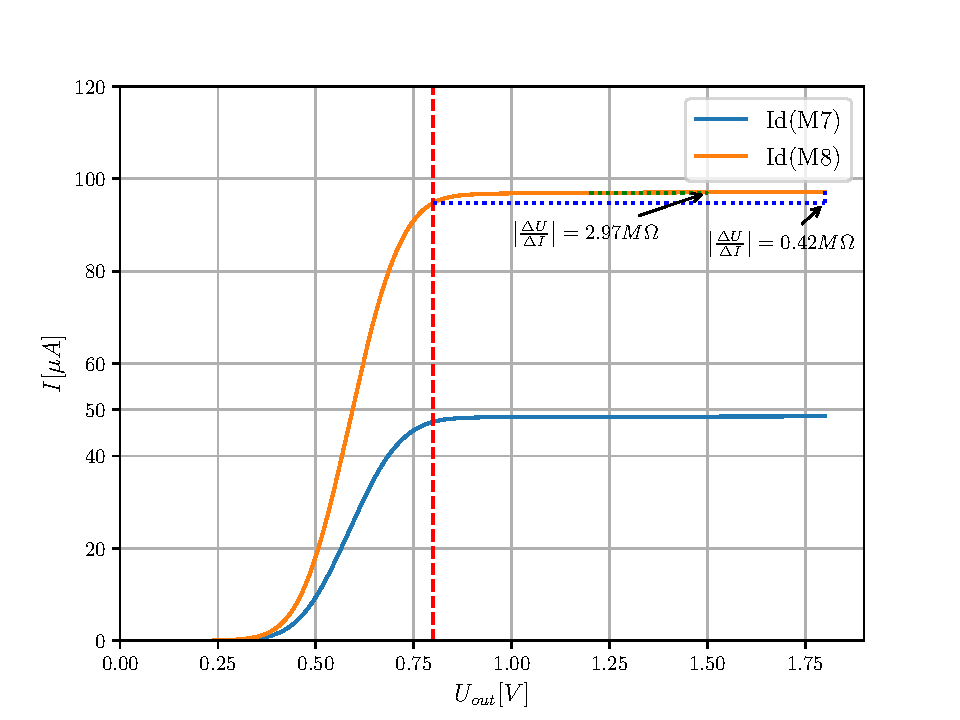
\includegraphics[width=0.8\textwidth]{2-3.pdf}
    \caption{DC analýza pro modifikované Wilsonovo proudové zrcadlo.}
    \label{fig:2-3-pdf}
\end{figure}


\clearpage
\section{Závěr}
  V této úloze jsme porovnávali tři základní typy proudových zrcadel. 

  Vždy byl proveden ruční výpočet parametrů součástek a výsledek byl následně prověřen simulací. Pro jednuduché proudové zrcadlo odpovídá výsledek simulace očekáváním -- zapojení je jednoduché a výpočet mohl být proveden poměrně přesně. Jak je vidět z grafu \ref{fig:2-1-pdf}, dynamický rozsah je přibližně \qty{1.6}{V}, napříč tímto rozsahem hodnota výstupního proudu přibližně lineárně roste z důvodu efektu modulace délky kanálu.

  Pro kaskodové zrcadlo se simulace poměrně odchyluje od požadavků na vstupní a výstupní proud, ruční výpočet byl tedy méně přesný. Hodnoty použité v ručním výpočtu pocházejí z tabulek z první úlohy, kdy jsme simulovali změny prahového napětí. Tyto tabulky neobsahují hodnoty pro požadovaný poměr \(W/L\) ani pro napětí na bulku horního tranzistoru. Byly tedy použity hodnoty nejbližší, nikoliv zcela přesné, tím mohlo dojít k chybě. Z výsledků simulace plyne, že největší chyba je u výpočtu hodnoty rezistoru. Pokud bychom použili přesnější hodnoty a nebo iterovali v rámci simulace, dojdeme k podstatně lepšímu výsledku. Dynamický rozsah tohoto zapojení je o něco málo menší, přibližně \qty{1.55}{V}. Výstupní odpor je ale oproti jednoduchému zrcadlu podstatně vyšší, výstupní proud tedy není tolik závislý na změně výstupního napětí.

  Pro Wilsonovo zrcadlo opět došlo k odchylce simulovaných proudů od hodnoty, se kterou pracuje výpočet. Důvod je stejný jako v předchozím případě. Jako výchozí bod návrhu jsou ale i tyto výpočty dostatečně přesné. U Wilsonova zrcadla vychází výstupní odpor výrazně nižší než u zrcadla kaskodového (vypočtená hodnota je pak ještě nižší než simulovaná), dynamický rozsah je také menší a to přibližně \qty{1}{V}. 

\begin{table}[h!]
  \centering
  \def\arraystretch{1.2}
  \begin{tabular}{|l||ll||ll||ll|}
  \hline
                    & \multicolumn{2}{l||}{Jednuduché} & \multicolumn{2}{l||}{Kaskodové} & \multicolumn{2}{l|}{Wilsonovo} \\ \hline
                    & \multicolumn{1}{l|}{V} & S & \multicolumn{1}{l|}{V} & S & \multicolumn{1}{l|}{V} & S \\ \hline\hline
  Vstupní proud [\unit{\micro\ampere}]  & \multicolumn{1}{l|}{25}  &  25 & \multicolumn{1}{l|}{50}  & 54  & \multicolumn{1}{l|}{50}  & 49  \\ \hline
  Výstupní proud [\unit{\micro\ampere}] & \multicolumn{1}{l|}{50}  &  50 & \multicolumn{1}{l|}{100}  &  109 & \multicolumn{1}{l|}{100}  &  97 \\ \hline
  \(r_{OUT} \)  [\unit{\mega\ohm}]          & \multicolumn{1}{l|}{\num{0.455}}  &  \num{0.4} & \multicolumn{1}{l|}{\num{16}}  & 16  & \multicolumn{1}{l|}{\num{0.9}}  &  3 \\ \hline
  \end{tabular}
  \caption{Porovnání hodnot simulace (S) a ručních výpočtů (V).}
  \label{tab:1-1-2_hodnoty}
  \end{table}
% \section*{Reference}
% \printbibliography[heading=none]


\end{document}